\documentclass{article}
\usepackage{listings}
\usepackage{graphicx}
\usepackage{hyperref}
\usepackage{url}
\usepackage{tocbibind}

\title{Smart Calculator}
\author{Dmitriy}
\date{\today}

\begin{document}

\maketitle
\tableofcontents
\clearpage

\section{Introduction}
\begin{enumerate}
  \item The program is developed in standard C11 using the gcc compiler and QT modules.
  \item Assembly of the program is configured using Makefile with a set of goals: all, install, uninstall, clean, dvi, dist, test, gcov report.
  \item The calculator has the ability to calculate arithmetic expressions, taking into account the priorities, as well as some mathematical functions (sine, cosine, logarithm, etc.).
  \item In addition to calculating expressions, the calculator also supports the use of the variable x and the construction of the graph of the corresponding function.
\end{enumerate}

\section{Install}
Follow these steps to install the calculator:
\begin{enumerate}
  \item Unpack the archive on your computer.
  \item Navigate to the directory with the extracted code.
  \item Install the program with the command \texttt{make install}.
  \item Run the calculator.
\end{enumerate}

\section{Screenshots}
\begin{figure}[htbp]
  \centering
  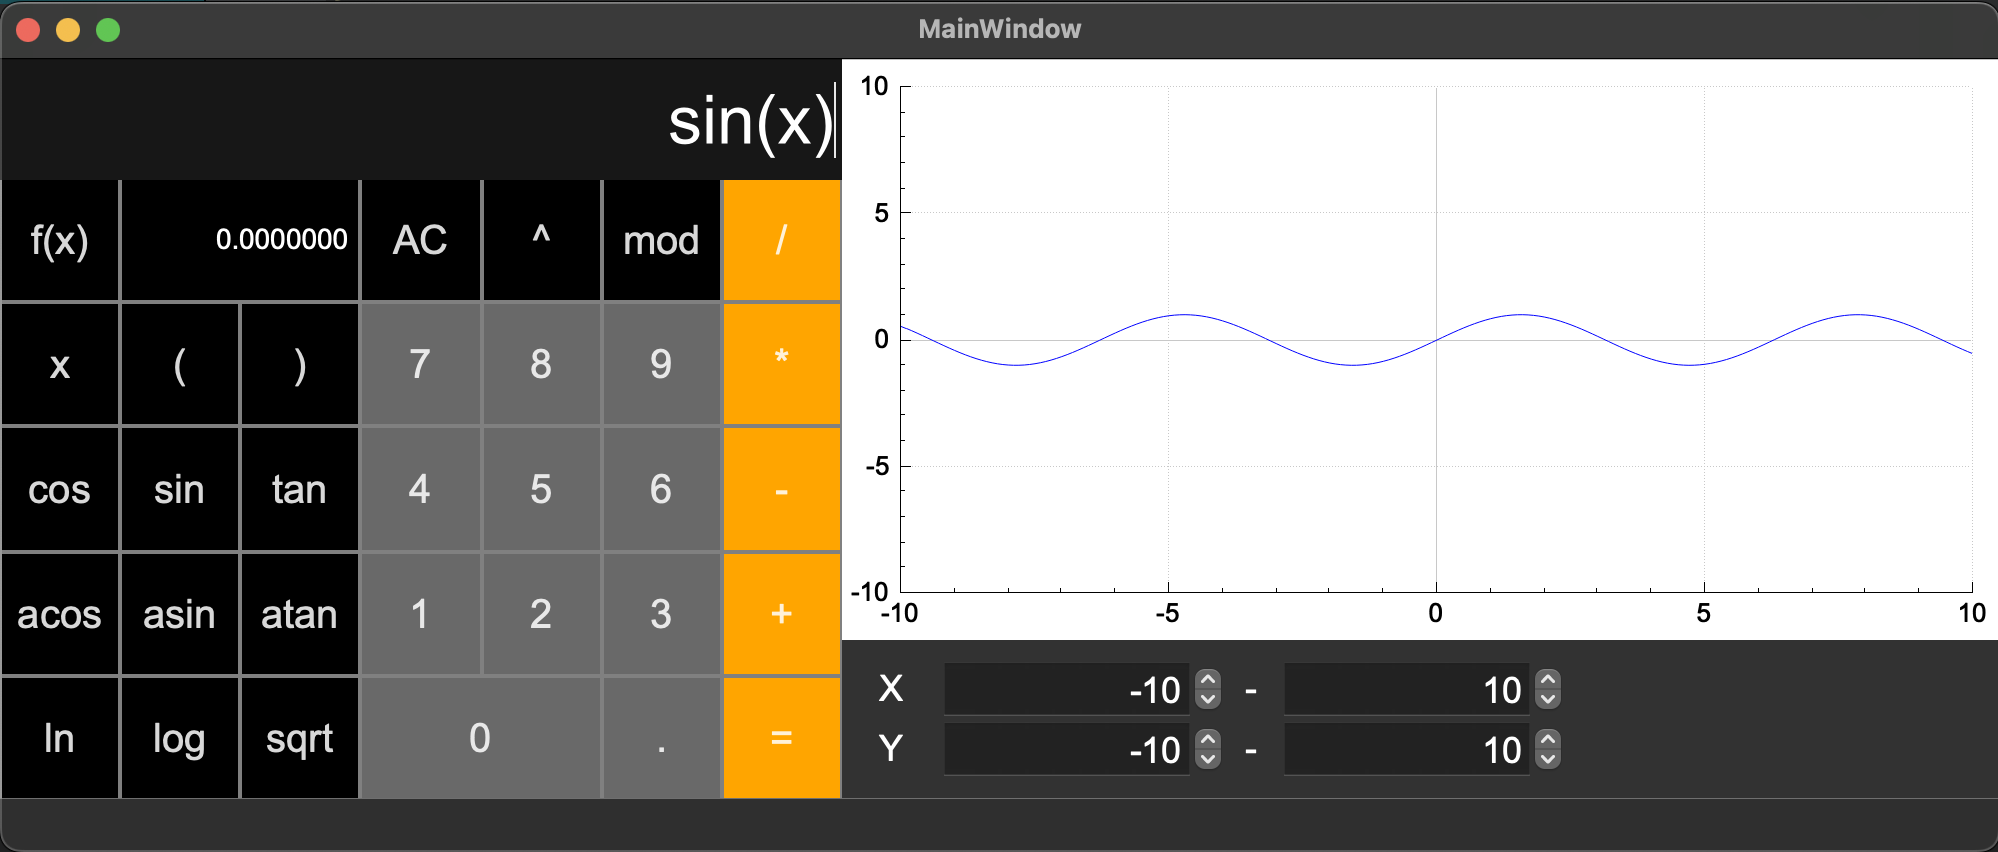
\includegraphics[width=0.8\textwidth]{screenshots/screenshot1.png}
  \caption{The workspace of the calculator}
  \label{fig:screenshot1}
\end{figure}

\clearpage
\section{Parsing code}

\begin{lstlisting}[language=C]

void to_polish_not(const char *strin, char *strout) {
  Stack stack;
  stack.top = NULL;
  int i, j = 0;
  for (i = 0; strin[i] != '\0'; i++) {
    if (isdigit(strin[i])) {  // the input symbol refers to digits
      while (isdigit(strin[i]) || strin[i] == '.') {
        strout[j++] = strin[i++];
      }
      strout[j++] = ' ';
      --i;
    } else if (strin[i] == '(' ||
               is_func(strin[i])) {  // the input symbol refers to functions
      push(&stack, strin[i]);
    } else if (strin[i] == ')' || strin[i] == ',') {
      while (!is_empty(&stack) && peek_operator(&stack) != '(') {
        strout[j++] = pop_operator(&stack);
        strout[j++] = ' ';
      }
      if (!is_empty(&stack) && peek_operator(&stack) == '(') {
        pop_operator(&stack);
      }
      if (!is_empty(&stack) && is_func(peek_operator(&stack))) {
        strout[j++] = pop_operator(&stack);
        strout[j++] = ' ';
      }
    } else if (is_operator(strin[i])) {  // the input symbol refers to operators
      while (!is_empty(&stack) && peek_operator(&stack) != '(' &&
             (priority(strin[i]) <= priority(peek_operator(&stack)))) {
        strout[j++] = pop_operator(&stack);
        strout[j++] = ' ';
      }
      push(&stack, strin[i]);
    }
  }
  while (!is_empty(&stack)) {
    strout[j++] = pop_operator(&stack);
    strout[j++] = ' ';
  }
  strout[j] = '\0';
}

\end{lstlisting}

\end{document}
